\chapter{Evaluation}
\label{chapter:evaluation}
% This is where Assessors will be looking for signs of success and for evidence of thorough and systematic evaluation as discussed in Section 8.3. Sample output, tables of timings and photographs of workstation screens, oscilloscope traces or circuit boards may be included. A graph that does not indicate confidence intervals will generally leave a professional scientist with a negative impression.
% As with code, voluminous examples of sample output are usually best left to appendices or omitted altogether.
% There are some obvious questions which this chapter will address. How many of the original goals were achieved? Were they proved to have been achieved? Did the program, hardware, or theory really work?
% Assessors are well aware that large programs will very likely include some residual bugs. It should always be possible to demonstrate that a program works in simple cases and it is instructive to demonstrate how close it is to working in a really ambitious case.

% ~2,000 words

\section{Model ranking and selection}
\label{section:model-ranking}
Following the hyperparameter tuning process described in Section~\ref{section:training-procedure}, the models were selected according to the following procedure (applied separately to the GCN and GAT model families):
\begin{enumerate}
    \item First, the models were ranked by ascending average MSE loss. The model with the lowest average MSE was chosen as the reference model.
    \item All models whose 1 standard deviation interval from their MSE did not overlap with the 1 standard deviation interval of the reference model MSE were excluded from ranking.
\end{enumerate}

The cross-validation performance of the best-scoring models selected by the above procedure is shown in Figure~\ref{figure:gat-gcn-rank}. The hyperparameters for each of the short-listed models are listed in Tables~\ref{table:shortlisted-gcn} and~\ref{table:shortlisted-gat} (Appendix~\ref{appendix:hyperparameters}).

% \begin{figure}[]
%     \centering
%     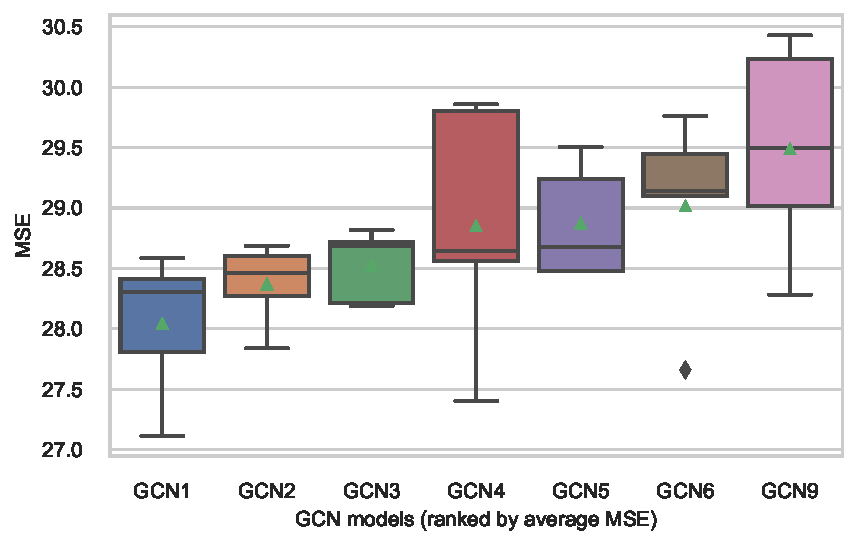
\includegraphics[width=\textwidth]{gcn_model_selection.pdf}
%     \caption{Highest scoring population graph and GCN model parameter combinations.}\label{figure:gcn-rank}
% \end{figure}

% \begin{figure}[]
%     \centering
%     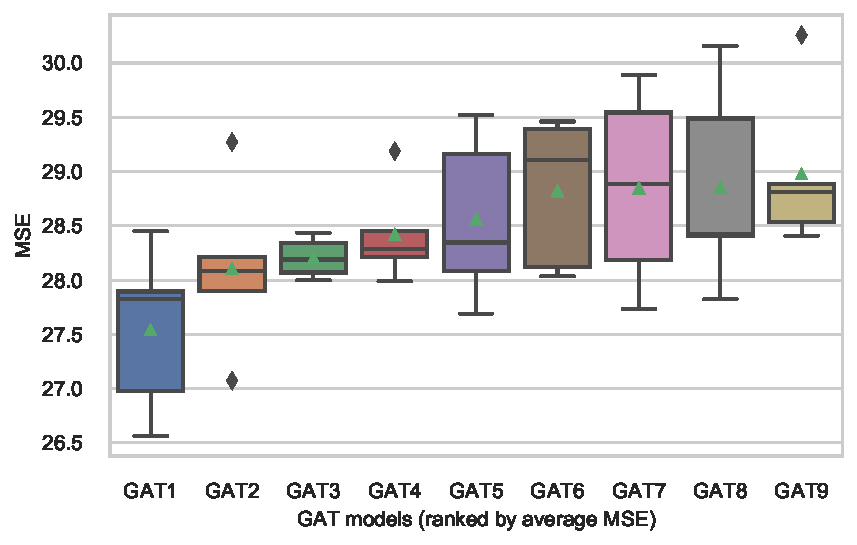
\includegraphics[width=\textwidth]{gat_model_selection.pdf}
%     \caption{Highest scoring population graph and GAT model parameter combinations.}\label{figure:gat-rank}
% \end{figure}

\begin{figure}[h]
    \centering
    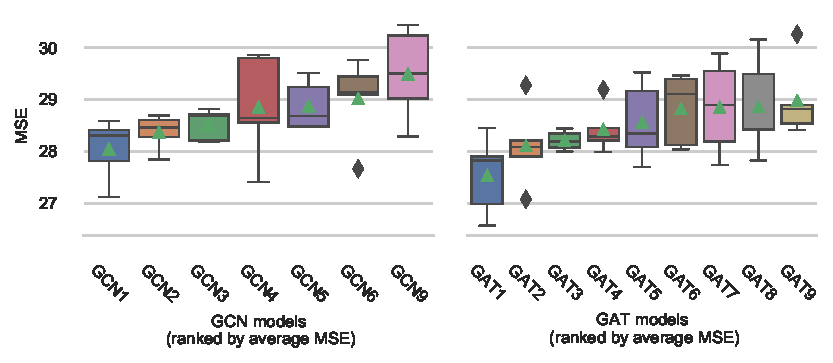
\includegraphics[width=\textwidth]{model_selection.pdf}
    \caption{Highest scoring population graph and GNN model parameter combinations.}\label{figure:gat-gcn-rank}
\end{figure}

Although both best-ranked (reference) models (GCN1 and GAT1) have relatively high variance, they still seem to be the most promising and therefore have been selected for further evaluation. Their population graph specification and GNN architecture hyperparameters are listed in Table~\ref{table:best-hyperparameters}.

\begin{table}[]
    \caption{Best performing population graph and GNN model parameter combinations during the model selection process.}\label{table:best-hyperparameters}
    \centering
    \small
    \begin{tabular}{p{0.3\textwidth}p{0.3\textwidth}p{0.3\textwidth}}
        \hline
    \textbf{Hyperparameter} & \textbf{GCN1} & \textbf{GAT1} \\  \hline
        Similarity feature set & \texttt{FI}, \texttt{FTE}, \texttt{ICD10}, \texttt{MEM}, \texttt{SEX} & \texttt{FI}, \texttt{ICD10}, \texttt{MEM}, \texttt{SEX} \\
        Similarity threshold & 0.9 & 0.8 \\ \hline
        Layer sizes & [1024, 512, 512, 256, 256, 1] & [2048, 1024, 512, 256, 128, 1] \\
        \# convolutional layers & 5 & 2 \\
        Dropout & $3.22 \times 10^{-1}$ & $3.14 \times 10^{-3}$ \\
        Learning rate & $6.98 \times 10^{-3}$ & $1.34 \times 10^{-2}$ \\
        Weight decay & $1.31 \times 10^{-2}$ & $6.05 \times 10^{-4}$ \\ \hline
\end{tabular}
\end{table}

\section{Evaluation metrics}
\label{section:evaluation-metrics}
The main performance metrics used for most regression problems, including brain age estimation task, are \textit{Pearson's correlation} and \textit{coefficient of determination}.

\subsubsection{Pearson's correlation}
For sets of true labels $\mathbf{y}  = [y_1 \dots y_N]$ with mean $\bar{y}$ and predicted labels $\mathbf{\hat{y}} = [\hat{y}_1 \dots \hat{y}_N]$, \textit{Pearson's correlation} is computed as

\begin{equation}
    r(\mathbf{y}, \mathbf{\hat{y}}) = \frac{\mathrm{cov}(\mathbf{y}, \mathbf{\hat{y}})}{\sigma_{\mathbf{y}} \sigma_{\mathbf{\hat{y}}}},
\end{equation}

where $\mathrm{cov}(\cdot, \cdot)$ denotes covariance and $\sigma$ stands for standard deviation. 

\subsubsection{Coefficient of determination}
The \textit{coefficient of determination} indicates how much variance in the features $\mathbf{X}$ could be explained by the model. It is computed as 
\begin{equation}
    r^2 = 1 - \frac{\sum_{i} (y_i - \bar{y})^2}{\sum_{i} (y_i - \hat{y}_i)^2}.
\end{equation}

Higher values for both metrics (with maximum 1) indicate a higher level of agreement between the true and predicted labels and therefore higher predictive power.


\section{Test set performance of selected models}
Generally in literature, after using cross-validation for model selection, the model is retrained on the entire dataset before giving a point estimate on a hold-out test set~\cite{raschka2018model}. This is because training on more data, especially when the dataset is small, allows to learn more patterns and therefore give better predictions on the unseen data. However, in this project the validation set was also used for early stopping since neural networks are especially prone to overfitting~\cite{prechelt1998automatic}. Some investigation of the hyperparameter tuning has shown that applying the stopping criteria discussed in Section~\ref{section:training-procedure} on just the training set would have still led to convergence only after the model has already overfit on the unseen validation labels. On the other hand, it is unclear how the stopping criteria should be adjusted when the training set size increases. 

Considering that the UKB dataset is large and that retraining the model with more data but without early stopping might not pay off for the loss in generalisation, all cross-validation folds were kept for test set performance estimation. Table~\ref{table:test-performance} gives the hold-out test set estimates for the metrics discussed in Section~\ref{section:evaluation-metrics}.

\begin{table}[h]
    \caption{Test set performance of GCN and GAT models.}\label{table:test-performance}
    \centering
    \small
    \begin{tabular}{ccc}
        \hline
    \textbf{Model} & $r$ & $r^2$ \\  \hline
        GCN1 & $0.675 \pm 0.008$ & $0.445 \pm 0.010$ \\
        GAT1 & $0.670 \pm 0.005$ & $0.477 \pm 0.008$ \\ \hline
\end{tabular}
\end{table}


\section{Significance testing of model performance}
\subsection{Experimental setup}
A classical test for assessing whether the models have truly learnt the relationships between the input features and the response variable is called a \textit{permutation test}~\cite{ojala2010permutation}. The null hypothesis assumes that features and labels are independent (i.e. that there is no relationship between the neuroimaging and non-imaging data and brain age), and the distribution corresponding to this hypothesis is estimated by randomly permuting the labels in the dataset. The $p$-value for this test is computed as

\begin{equation}
    p = \frac{\sum_{i=1}^k \mathbf{1}\left[\mathcal{L}(\mathbf{\hat{y}}, \pi(\mathbf{y})) \leq \mathcal{L}(\mathbf{\hat{y}}, \mathbf{y})\right] + 1}{k+1}\label{eq:p-value}
\end{equation}

where $\mathcal{L}(\cdot, \cdot)$ error function used to train the model (in this project MSE), $\pi(\cdot)$ indicates a permutation function which uniformly returns a random permutation of the argument, and $k$ is the number of samples.

In this project, $k=1000$ samples will be taken for each model family and the results will be claimed significant if the $p$-value in Equation~\eqref{eq:p-value} falls below the significance level $\alpha=0.05$. 

\subsection{Results}
The null distributions of GCN and GAT model errors with permuted labels are shown in Figure~\ref{figure:permutation-test}, with the MSE for the original dataset indicated by the red line.

\begin{figure}[h]
    \centering
    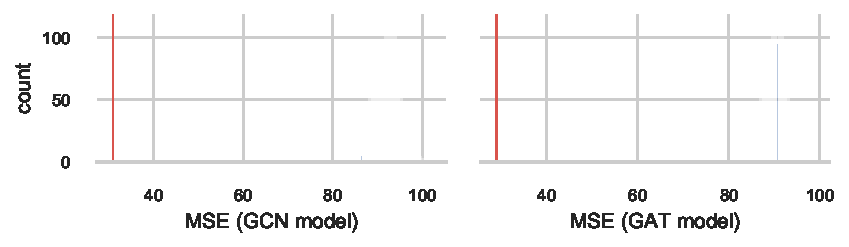
\includegraphics[width=\textwidth]{permutation_test.pdf}
    \caption{The null distribution of the label permutation test for GCN and GAT models. The red lines indicate MSE for the original dataset.}\label{figure:permutation-test}
\end{figure}

The $p$-values, representing how likely it is to get the MSE lower than the original dataset MSE purely by chance, were equal to $p=0.001$ for both GNN models. This is lower than the chosen significance level $\alpha=0.05$ so the null hypothesis is rejected and the performance of both models is statistically significant.


\section{GNN robustness to noisy population graph features}
\label{section:node-noise}
A desirable property for the real-world machine learning models is their robustness, defined as tolerance to the noise and inconsistency in data.
For example, as discussed in Section~\ref{section:implementation-robustness}, it is useful if the model can retain its performance even when the data contains particularly noisy MRI scans. Population graphs trained on graph neural networks could do this by exploiting the neighbourhoods that are hopefully less noisy than a given node. Whether they are actually capable of doing so could be tested by adding noise to an increasing proportion of nodes. 

\subsection{Experimental setup}
For the feature noise robustness evaluation, an increasing proportion of population graph nodes is corrupted by randomly permuting their features. Then the model is retrained and tested on the hold-out test set, measuring the change in performance. To make sure that any effect on the evaluation metrics is due to added noise and not the changing dataset split, the model is trained on a single dataset split while the noise is added to different subjects. Moreover, to ensure that the effect on test set performance is due to the interaction with neighbourhoods and not due to the individual node features, only the nodes in the training set will be corrupted. For each of the GCN and GAT models, the experiment is repeated five times for each noise level (1\%, 5\%, 10\%, 20\%, 30\%, 50\%, 80\%, and 95\% of training nodes).

\subsection{Results}

The results of corrupting the node features on the predictive power of GNN models are shown in Figure~\ref{figure:node-noise}.

% \begin{figure}[h]
%     \centering
%     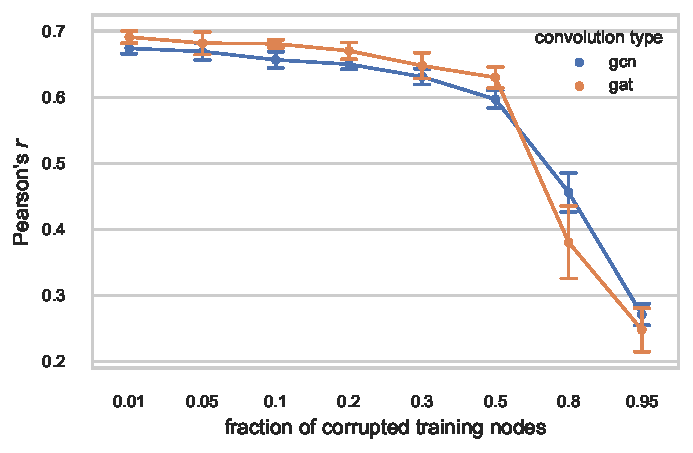
\includegraphics[]{node_noise_r.pdf}
% %     \caption{The effect of permuting node features on $r$ performance metric, with error bars representing standard deviation}\label{figure:node-noise-r}
% % \end{figure}

% % \begin{figure}[h]
% %     \centering
%     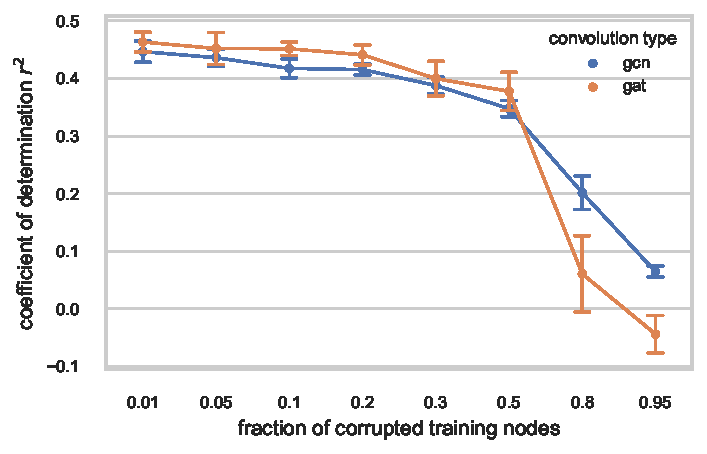
\includegraphics[]{node_noise_r2.pdf}
%     \caption{The effect of permuting node features on $r$ and $r^2$ performance metrics, with error bars representing standard deviation.}\label{figure:node-noise}
% \end{figure}

\begin{figure}[h]
    \centering
    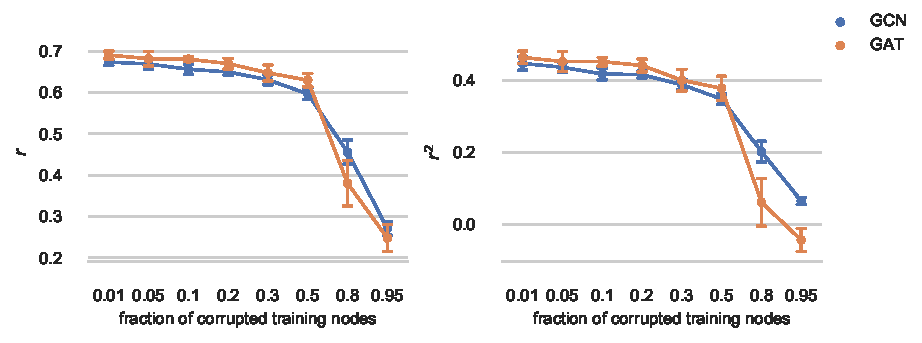
\includegraphics[]{node_noise.pdf}
    \caption{The effect of permuting node features on $r$ (left) and $r^2$ (right) performance metrics, with error bars representing standard deviation.}\label{figure:node-noise}
\end{figure}

As expected, for both GCN and GAT models the performance was decreasing relatively slowly as more training nodes got corrupted, and then dropped drastically when more than half of the training nodes had their features permuted. In case of the GAT model, the $r^2$ metric even fell below 0 (bottom of Figure~\ref{figure:node-noise}), which means that no variance could be explained and that the mean of the observed subject ages in the dataset is a better estimate of the brain age than the prediction of the GAT model. 

It is also possible to compare the relative GCN and GAT performance. While in this experiment the GAT model has higher (but similar) average scores at low noise levels, its performance drops faster, creating a wider gap between the scores, which could suggest that the GAT model is less robust to increasing noise. 

\subsection{Discussion}
In practice, in a big and well-curated dataset such as the UK Biobank, the existence of exact protocols for equipment and measurement taking should prevent there being too many unacceptably noisy scans. Even in that case, the noise would take a milder form than the complete shuffling of features that make the node data meaningless. Having that considered, at low proportions of added noise, both models have been able to retain most of their predictive power, which could indicate their generalisability to new contexts.


\section{GNN dependence on population graph similarity metrics}
\subsection{Experimental setup}
The assumption behind the population graph model is that the edge structure helps to control for confounding effects while giving additional information which could be useful for brain age prediction. One experiment to test this is to remove an increasing proportion of edges from the population graph, with the proportions of removed edges being the same as in the previous section. The training procedure is then repeated five times at each edge loss level using a different random seed. The more edges are removed, the less neighbourhood structure the graph neural network models can exploit, having to rely on individual node features. 

\subsection{Results}
The effect of removing the edges on predictive power of the GNN models is shown in Figure~\ref{figure:edge-noise}. Compared to the results in Section~\ref{section:node-noise} where the predictive power drastically dropped with increased noise, the loss of information contained in edges and neighbourhoods of similar nodes did \texttt{not} affect the predictive power of the models. This could be inferred from the standard deviation intervals being quite wide for both evaluation metrics, overlapping across most, if not all, edge loss levels.

% \begin{figure}[]
%     \centering
%     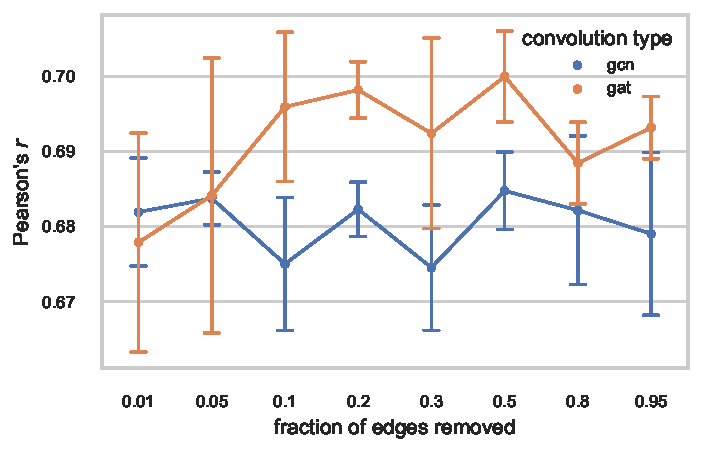
\includegraphics[]{edge_noise_r.pdf}
% %     \caption{The effect of removing edges on $r$ performance metric, with error bars representing standard deviation}\label{figure:edge-noise-r}
% % \end{figure}

% % \begin{figure}[h]
% %     \centering
%     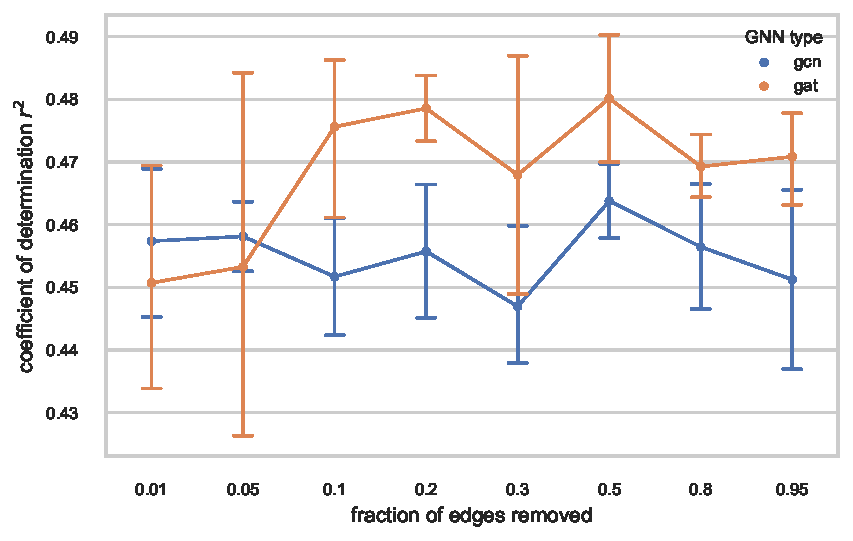
\includegraphics[]{edge_noise_r2.pdf}
%     \caption{The effect of removing edges on $r$ and $r^2$ performance metrics, with error bars representing standard deviation.}\label{figure:edge-noise}
% \end{figure}

\begin{figure}[h]
    \centering
    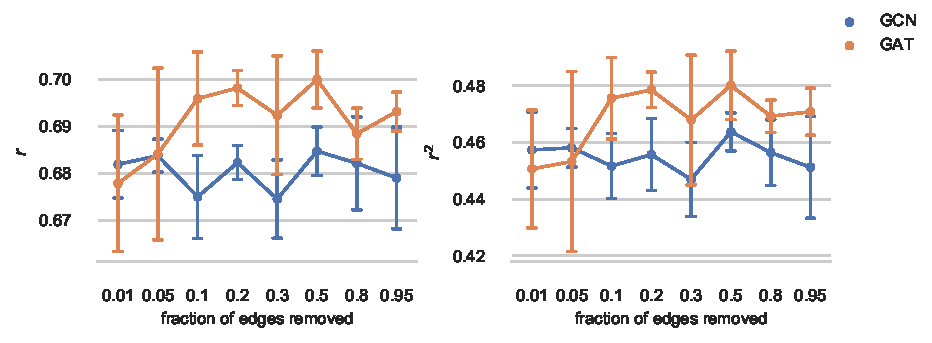
\includegraphics[]{edge_noise.pdf}
    \caption{he effect of removing edges on $r$ (left) and $r^2$ (right) performance metrics, with error bars representing standard deviation.}\label{figure:node-noise}
\end{figure}


\section{Discussion}
 The edge removal experiment shows that for brain age estimation problem, the models relied more on the features of individual nodes rather than similarity metrics and in turn the neighbourhoods of other population graph nodes. This might mean that the similarity metrics were not informative enough to allow for effective sharing of feature and/or label information, or that the (brain) age depends more on the feature interactions within a single brain rather than particular signals that generalise to other individuals. Moreover, the node noisification experiment shows that the neighbours could be even \textit{harmful} as, due to experimental setup, the changes in performance in Figure~\ref{figure:node-noise} are only due to the changes in neighbouring nodes but not in the test nodes themselves.

If this is true, more powerful models that do not use the graph structure might be more appropriate for the brain age estimation task. This is consistent with considerably better brain age estimation performance of other non-GNN models found in literature (such as $r=0.93$ in Kaufmann et al.~\cite{kaufmann2019} using an XGBoost model, and $r=0.94, r^2=0.88$ in Cole et al.~\cite{cole2018brain} using a Gaussian process regression model), and even ``consistently poor'' performance of GNN models when applied to a similar task (to the point that in Pervaiz et al.~\cite{pervaiz2020optimising} the GNN results were dropped altogether from further discussion).


% \section{Comparison against existing benchmarks}

% Compare to the Kaufmann et al.'s \textit{xgboost} approach \cite{kaufmann2019} ($r \sim 0.93$); and the other package that was cited in the same paper.
% Possibly compare to other non-graph (relatively baseline) (neural network) architectures, e.g. ElasticNet, MLP,...

